\section{Rezultaty i wnioski}

<Podrozdziały: "Funkcjonowanie algorytmu G-średnich", "Funkcjonowanie algorytmu SVM">

Pomiary czasu wykonywania programów napisanych w poszczególnych językach dla różnych paczek danych z bazy MIT-BIH zostały przedstawione w Tab.\ref{tabResults}.

\begin{table}[!tp]
	\centering
	\caption{Czasy wykonywania programu w poszczególnych językach dla różnych paczek danych. Wyniki wyrażone w sekundach}
	\label{tabResults}
	\begin{tabular}{|c|c|c|c|c|}
		\hline
		Nr paczki z MIT-BIH & C++ & Matlab & Python & Julia\\ \hline		
		100 & & 1.9523 & 12.8154 & 5.9018\\ \hline
		101 & & 1.4195 & 10.4921 & 1.8999\\ \hline
		102 & & 1.2609 & 12.2421 & 2.2158\\ \hline
		103 & & 2.3951 & 11.7082 & 2.1799\\ \hline
		104 & & 1.6457 & 11.8959 & 2.1335\\ \hline
		105 & & 1.3186 & 14.7023 & 3.1231\\ \hline
		106 & & 1.8217 & 10.3659 & 2.1148\\ \hline
		107 & & 1.5331 &  9.9881 & 2.0690\\ \hline
		108 & & 1.7391 &  8.5037 & 2.1076\\ \hline
		109 & & 1.2506 & 13.9100 & 3.4216\\ \hline
		111 & & 1.8369 & 11.5751 & 2.8740\\ \hline
		112 & & 2.2931 & 14.7076 & 3.3450\\ \hline
		113 & & 1.2857 & 10.2796 & 1.9383\\ \hline
		114 & & 0.5056 &  5.5475 & 1.5342\\ \hline
		115 & & 1.2325 & 11.0597 & 2.2074\\ \hline
		116 & & 1.242  & 13.3443 & 2.5876\\ \hline
		117 & & 1.506  &  8.4621 & 1.6436\\ \hline
		119 & & 1.5771 & 10.9920 & 2.0712\\ \hline
		121 & & 2.0902 & 10.2799 & 1.9764\\ \hline
		122 & & 2.0928 & 14.2113 & 3.1178\\ \hline
		123 & & 0.7942 &  8.3969 & 1.7214\\ \hline
		124 & & 1.6778 &  8.1375 & 1.7144\\ \hline
		200 & & 1.8849 & 11.5171 & 2.8278\\ \hline
		201 & & 1.8963 &  9.2492 & 1.8645\\ \hline
		202 & & 2.132  & 13.7891 & 3.7783\\ \hline
		203 & & 1.2565 & 14.5795 & 3.1471\\ \hline
		205 & & 1.3475 & 15.0668 & 3.2602\\ \hline
		208 & & 2.4411 & 15.5730 & 3.5292\\ \hline
		209 & & 2.139  & 17.3970 & 4.0027\\ \hline	
		210 & & 1.1721 & 26.9134 & 6.4331\\ \hline
		212 & & 2.9475 & 26.8902 & 3.3900\\ \hline
		213 & & 2.3988 & 31.4794 & 4.1460\\ \hline
		214 & & 1.8288 & 18.5719 & 2.4208\\ \hline
		215 & & 1.6584 & 30.4394 & 3.9548\\ \hline
		217 & & 2.0103 & 18.7011 & 2.5876\\ \hline
		219 & & 1.8043 & 19.7484 & 3.2817\\ \hline
		220 & & 1.2670 & 18.7101 & 2.6659\\ \hline		
		221 & & 1.7631 & 13.7085 & 3.0061\\ \hline
		222 & & 1.2655 & 14.3837 & 3.2237\\ \hline
		223 & & 1.2356 & 13.7316 & 3.0060\\ \hline
		230 & & 1.8286 & 14.1915 & 2.8750\\ \hline
		231 & & 1.4458 &  8.6988 & 3.3912\\ \hline
		232 & & 1.3707 & 10.3213 & 2.3545\\ \hline
		233 & & 2.5759 & 15.5837 & 3.4775\\ \hline
		234 & & 3.6223 & 16.4921 & 3.5836\\ \hline
		\textbf{Czas średni} & - & 1.5836 & - & 2.3554\\ \hline
	\end{tabular}
\end{table}

\begin{table}[!tp]
	\centering
	\caption{Liczby klas wyliczonych przez G-means}
	\label{tabResults2}
	\begin{tabular}{|c|c|c|c|}
		\hline
		Nr paczki z MIT-BIH & Matlab & Python & Julia\\ \hline		
		100 & 16 & 16 & 16\\ \hline
		101 & 14 & 16 & 16\\ \hline
		102 & 14 & 16 & 16\\ \hline
		103 & 27 & 16 & 16\\ \hline
		104 & 29 & 16 & 16\\ \hline
		105 &  1 & 20 & 20\\ \hline
		106 & 35 & 16 & 16\\ \hline
		107 & 31 & 16 & 16\\ \hline
		108 & 32 & 15 & 15\\ \hline
		109 &  1 & 21 & 21\\ \hline
		111 & 22 & 17 & 17\\ \hline
		112 & 15 & 19 & 19\\ \hline
		113 & 13 & 16 & 16\\ \hline
		114 &  1 & 15 & 15\\ \hline
		115 & 15 & 16 & 16\\ \hline
		116 &  1 & 16 & 16\\ \hline
		117 & 23 & 16 & 16\\ \hline
		119 & 33 & 16 & 16\\ \hline
		121 & 27 & 16 & 16\\ \hline
		122 & 29 & 21 & 21\\ \hline
		123 &  1 & 16 & 16\\ \hline
		124 & 30 & 15 & 15\\ \hline
		200 & 32 & 20 & 20\\ \hline
		201 & 56 & 13 & 13\\ \hline
		202 & 29 & 21 & 21\\ \hline
		203 &  1 & 26 & 26\\ \hline
		205 &  1 & 21 & 21\\ \hline
		208 & 36 & 24 & 24\\ \hline
		209 & 21 & 31 & 31\\ \hline
		210 &  1 & 20 & 20\\ \hline
		212 & 18 & 25 & 25\\ \hline
		213 & 28 & 32 & 32\\ \hline
		214 & 33 & 18 & 18\\ \hline
		215 & 18 & 32 & 32\\ \hline
		217 & 65 & 17 & 17\\ \hline
		219 & 36 & 15 & 15\\ \hline
		220 & 22 & 16 & 16\\ \hline	
		221 & 33 & 19 & 19\\ \hline
		222 &  1 & 22 & 22\\ \hline
		223 &  1 & 18 & 18\\ \hline
		230 & 15 & 20 & 20\\ \hline
		231 & 39 & 12 & 12\\ \hline
		232 & 28 & 17 & 17\\ \hline
		233 & 42 & 24 & 24\\ \hline
		234 & 27 & 29 & 29\\ \hline
	\end{tabular}
\end{table}

Krótki czas wykonywania programu napisanego w Matlabie wynika głównie z wykorzystania biblioteki libsvm \cite{csie}, która jest napisana w C. Dla pozostałych języków zaimplementowano maszynę wektorów nośnych w oparciu o pliki źródłowe wspomnianej biblioteki.

Wykorzystanie metody SVM z szesnastoelementowym wektorem cech wydaje się złym rozwiązaniem, gdyż niemal zawsze wektor klasyfikowany jest do jednej klasy - patrz Rys.\ref{fig:hist1}. Poza zbyt licznym wektorem cech wpływ na to ma również fakt, że około 90\% zespołów QRS z bazy MIT-BIH reprezentują pobudzenia nadkomorowe. Rozwiązaniem problemu klasyfikacji może okazać się odpowiednie zmniejszenie liczności wykorzystywanego wektora cech.

Przeprowadzono również testy, w których SVM korzystał z różnych modeli (wygenerowanych z różnych paczek danych). Zaobserwowano, że normalizacja wektorów uczących znacznie przyspiesza proces uczenia, czego potwierdzeniem jest Rys.\ref{fig:SVM}.

\begin{figure}[!htp]
	\centering
	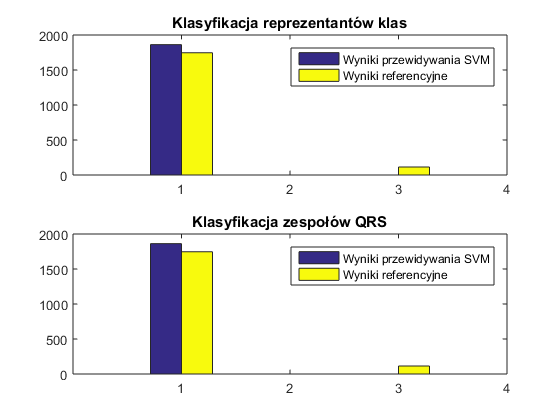
\includegraphics[width=15cm]{Grafika/101_2_3}
	\caption{Histogramy klasyfikacji zespołów dla paczki danych o numerze 101}
	\label{fig:hist1}
\end{figure}

\begin{figure}[!htp]
	\centering
	\includegraphics[width=16cm]{Grafika/SVMTrain}
	\caption{Wpływ normalizacji na czas nauki SVM}
	\label{fig:TrainNormSVM}
\end{figure}

<Coś o gmeans - że w C++ nie było, a tutaj jest>


%\begin{table}[H]
%\caption{Example table}
%\centering
%\begin{tabular}{llr}
%\toprule
%\multicolumn{2}{c}{Name} \\
%\cmidrule(r){1-2}
%First name & Last Name & Grade \\
%\midrule
%John & Doe & $7.5$ \\
%Richard & Miles & $2$ \\
%\bottomrule
%\end{tabular}
%\end{table}
